\documentclass{beamer}
\usetheme{Madrid}
\usecolortheme{default}

% ── Packages ──────────────────────────────────────────────────────────────────
\usepackage{graphicx}
\usepackage{booktabs}
\usepackage{amsmath}
\usepackage{xcolor}
\usepackage{tikz}
\usetikzlibrary{arrows.meta, positioning}

% ── Colors ────────────────────────────────────────────────────────────────────
\definecolor{uoftblue}{RGB}{6,41,88}
\definecolor{highlightblue}{RGB}{31,119,180}
\definecolor{highlightred}{RGB}{214,39,40}
\definecolor{highlightgreen}{RGB}{44,160,44}
\definecolor{lightgray}{RGB}{245,245,245}

\setbeamercolor{titlelike}{bg=uoftblue}
\setbeamerfont{title}{series=\bfseries}

% white background for all frames
\setbeamercolor{background canvas}{bg=white}
\setbeamercolor{normal text}{fg=black}

% ── Metadata ──────────────────────────────────────────────────────────────────
\title[LoFTR Distillation]{Lightweight Feature Matching via\\Knowledge Distillation from LoFTR}

\subtitle{ECE1508 Applied Deep Learning — Winter 2026}

\author[Chen, Li, Zhu]{%
  Jerry Chen \and Spiro Li \and Weijie Zhu}

\institute[UofT ECE]{%
  The Edward S.\ Rogers Sr.\ Department of Electrical \& Computer Engineering\\
  University of Toronto}

\date{April 2026}

\logo{
\includegraphics[height=0.8cm]{logo_uoft}}

% ══════════════════════════════════════════════════════════════════════════════
\begin{document}

% ── Slide 1: Title (does not count) ──────────────────────────────────────────
\frame{\titlepage}


% ── Slide 2: Motivation ──────────────────────────────────────────────────────
\begin{frame}
\frametitle{Motivation}

\textbf{Feature matching} is the foundation of visual localization, SLAM, and 3D reconstruction.

\vspace{0.6em}
\begin{columns}[T]
\begin{column}{0.48\textwidth}
  \textbf{LoFTR} (Sun et al., 2021)
  \begin{itemize}
    \item State-of-the-art detector-free matcher
    \item Transformer-based, \textbf{$\sim$12M} parameters
    \item Too heavy for mobile / edge deployment
  \end{itemize}
\end{column}
\begin{column}{0.48\textwidth}
  \textbf{Our Goal}
  \begin{itemize}
    \item Compress LoFTR via \textcolor{highlightblue}{\textbf{knowledge distillation}}
    \item Student models with $<$1M parameters
    \item \textcolor{highlightred}{\textbf{$\sim$20$\times$}} parameter reduction
  \end{itemize}
\end{column}
\end{columns}

\vspace{0.8em}
\centering
\textcolor{gray}{\textit{Can a tiny student learn LoFTR's matching ability?}}
\end{frame}


% ── Slide 3: Architecture ────────────────────────────────────────────────────
\begin{frame}
\frametitle{Student Architecture}

\begin{center}
  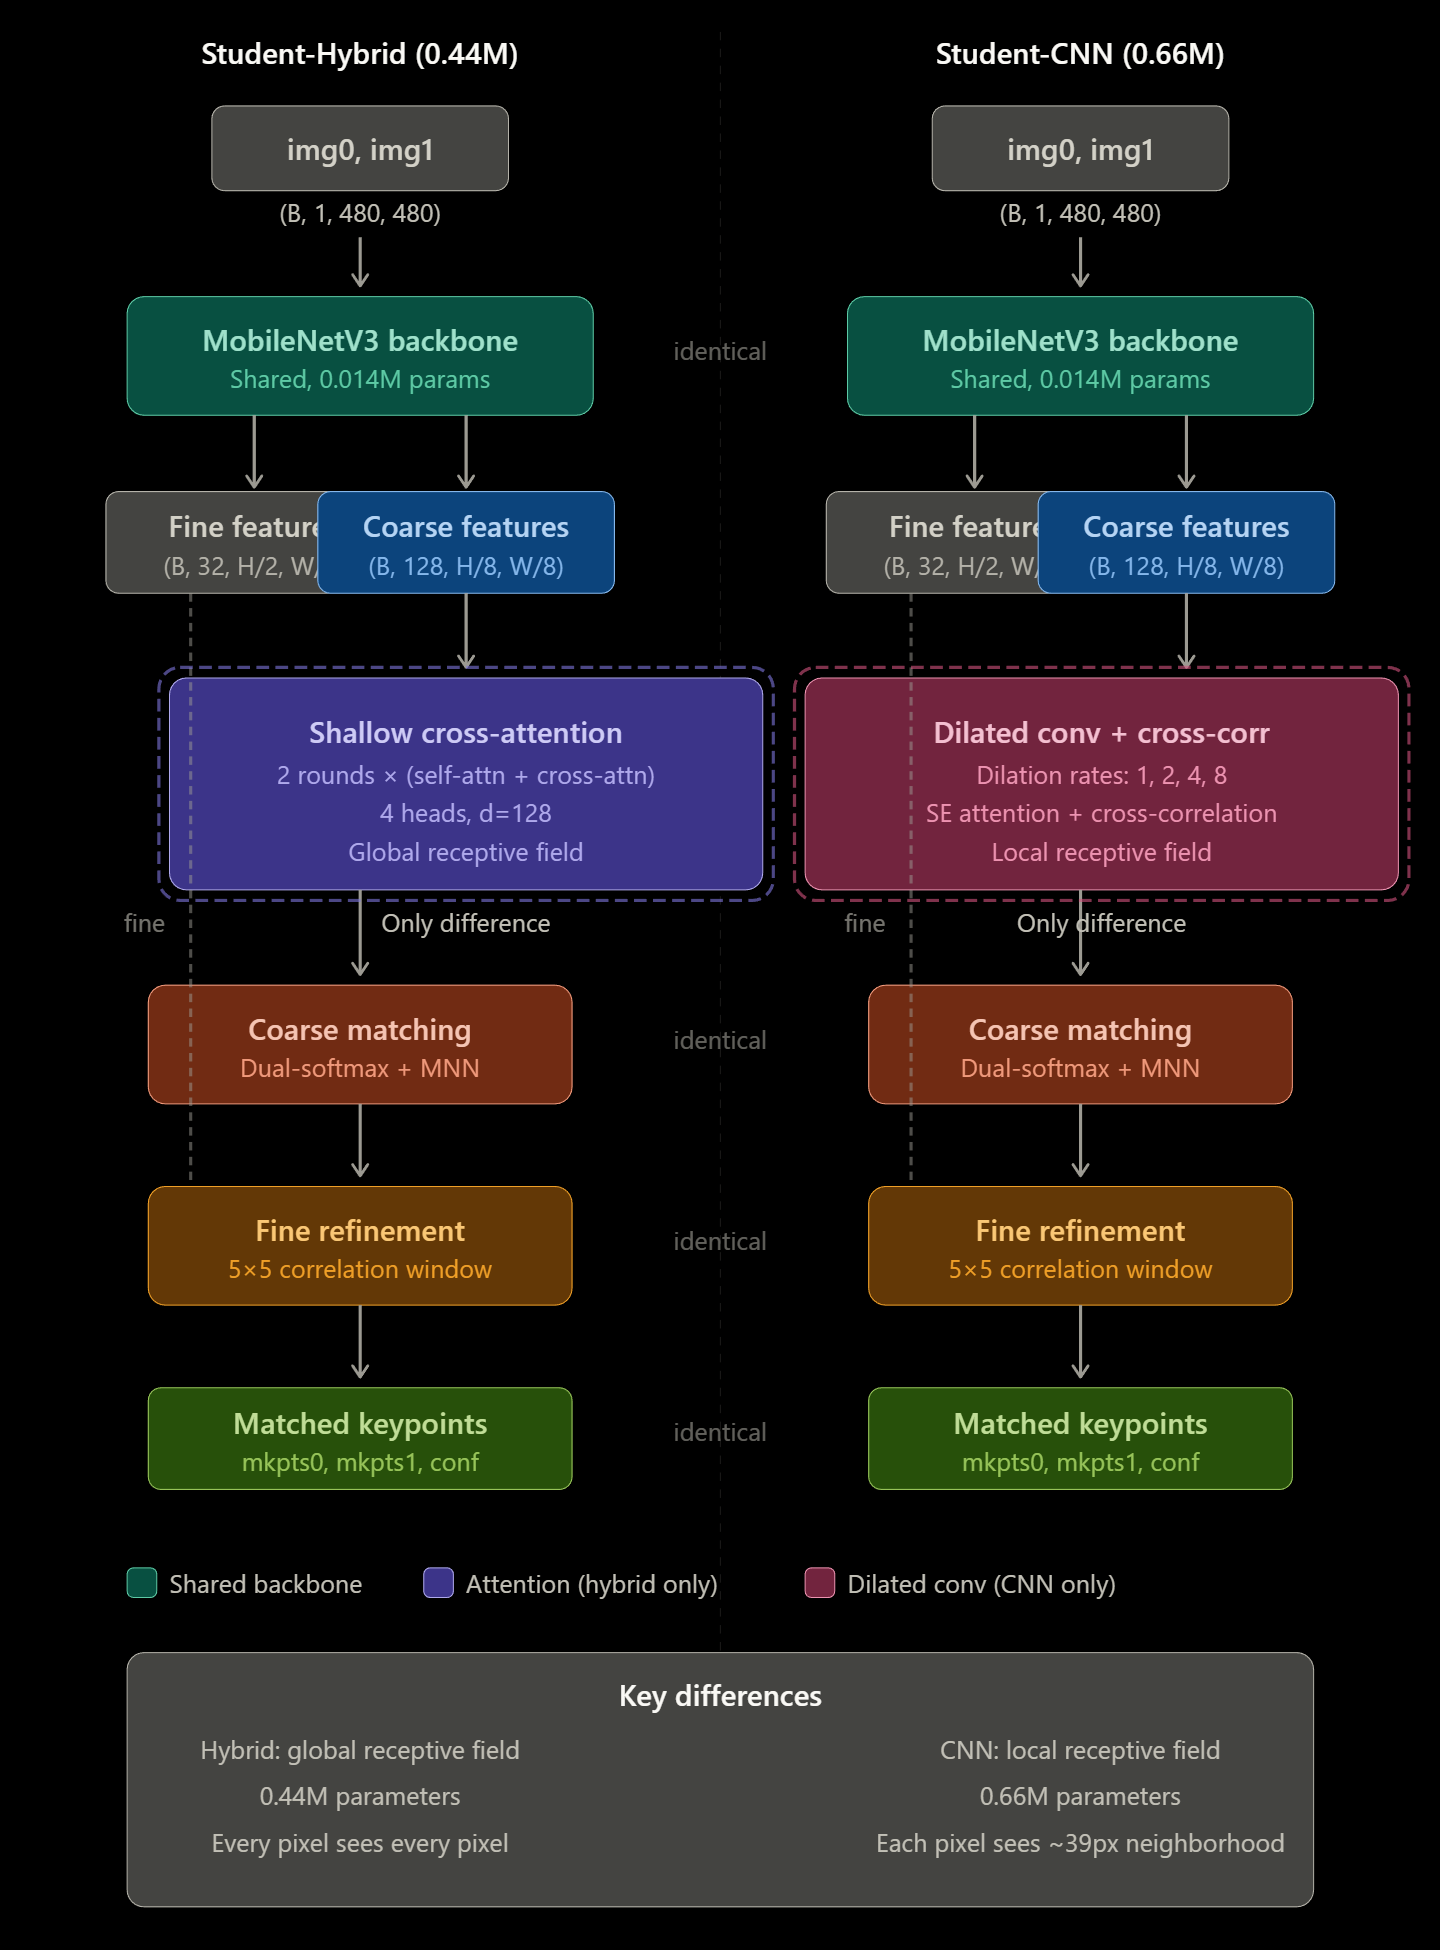
\includegraphics[width=0.9\textwidth,height=0.6\textheight,keepaspectratio]{structure.PNG}
\end{center}

\vspace{0.2em}
\small
\begin{columns}[T]
\begin{column}{0.48\textwidth}
  \centering
  \textcolor{highlightblue}{\textbf{Student-Hybrid (0.44M)}}\\
  Shallow cross-attention\\
  \textit{Global receptive field}
\end{column}
\begin{column}{0.48\textwidth}
  \centering
  \textcolor{highlightred}{\textbf{Student-CNN (0.66M)}}\\
  Dilated convolutions\\
  \textit{Local receptive field}
\end{column}
\end{columns}
\end{frame}


% ── Slide 4: Method + Results (merged) ───────────────────────────────────────
\begin{frame}
\frametitle{Method \& Results}

\scriptsize
\vspace{-0.5em}
$\mathcal{L}_{total} =
  1.0 \cdot \underset{\textcolor{highlightblue}{\text{KL div}}}{\mathcal{L}_{coarse}^{KD}}
+ 0.5 \cdot \underset{\textcolor{highlightgreen}{\text{MSE}}}{\mathcal{L}_{feat}^{KD}}
+ 1.0 \cdot \underset{\textcolor{highlightred}{\text{Focal}}}{\mathcal{L}_{GT}}$
\hfill
\textbf{Setup:} HPatches, 1k pairs/epoch, AdamW 3e-4, 20 ep \hfill Hybrid 0.44M \quad CNN 0.66M

\vspace{0.4em}
\centering
\footnotesize
\begin{tabular}{l ccc ccc}
  \toprule
  & \multicolumn{3}{c}{\textbf{Threshold = 0.2}} & \multicolumn{3}{c}{\textbf{Threshold = 0.02}} \\
  \cmidrule(lr){2-4} \cmidrule(lr){5-7}
  \textbf{Model} & @3 & @5 & @10 & @3 & @5 & @10 \\
  \midrule
  Hybrid (KD+GT) & \textcolor{highlightred}{0.00} & \textcolor{highlightred}{0.04} & \textcolor{highlightred}{0.33}
    & 12.65 & 24.03 & \textcolor{highlightgreen}{\textbf{36.17}} \\
  CNN (KD+GT) & 1.58 & 3.91 & 7.80
    & 12.59 & 22.59 & 34.34 \\
  \midrule
  Hybrid (GT-only) & 9.95 & 18.36 & 31.38
    & 9.95 & 18.36 & 31.38 \\
  CNN (GT-only) & \textcolor{highlightgreen}{\textbf{13.18}} & \textcolor{highlightgreen}{\textbf{22.70}} & \textcolor{highlightgreen}{\textbf{34.34}}
    & 13.18 & 22.70 & 34.34 \\
  \midrule
  LoFTR Teacher & 51.82 & 66.62 & 77.99
    & — & — & — \\
  \bottomrule
\end{tabular}

\vspace{0.4em}
\raggedright
\scriptsize
\begin{enumerate}
  \item \textcolor{highlightblue}{\textbf{Confidence calibration:}} KD flattens confidence $\Rightarrow$
        threshold 0.2 fails; at 0.02 Hybrid recovers to \textbf{36.17\%}
  \item \textcolor{highlightgreen}{\textbf{CNN $>$ Attention:}} CNN wins in most configs
        (more params, shallow attn too weak, local features suffice)
  \item \textcolor{highlightred}{\textbf{Gap:}} best student 36\% vs teacher 78\%
        (20$\times$ compression + synthetic data domain gap)
\end{enumerate}
\end{frame}


% ── Slide 6: Conclusions ─────────────────────────────────────────────────────
\begin{frame}
\frametitle{Conclusions \& Future Work}

\small
\textbf{Conclusions}
\begin{enumerate}
  \item KD \textbf{does transfer} matching knowledge, but requires \textcolor{highlightblue}{\textbf{confidence recalibration}}
  \item Convolutional student \textcolor{highlightgreen}{\textbf{outperforms}} shallow attention at this scale
  \item Training data quality is the \textcolor{highlightred}{\textbf{primary bottleneck}}, not architecture
\end{enumerate}

\vspace{0.2em}
\textbf{Future Work:}
\textbf{MegaDepth} real 3D data \quad|\quad deeper attention \quad|\quad learnable \textbf{confidence calibration layer}

\vspace{0.3em}
\begin{center}
  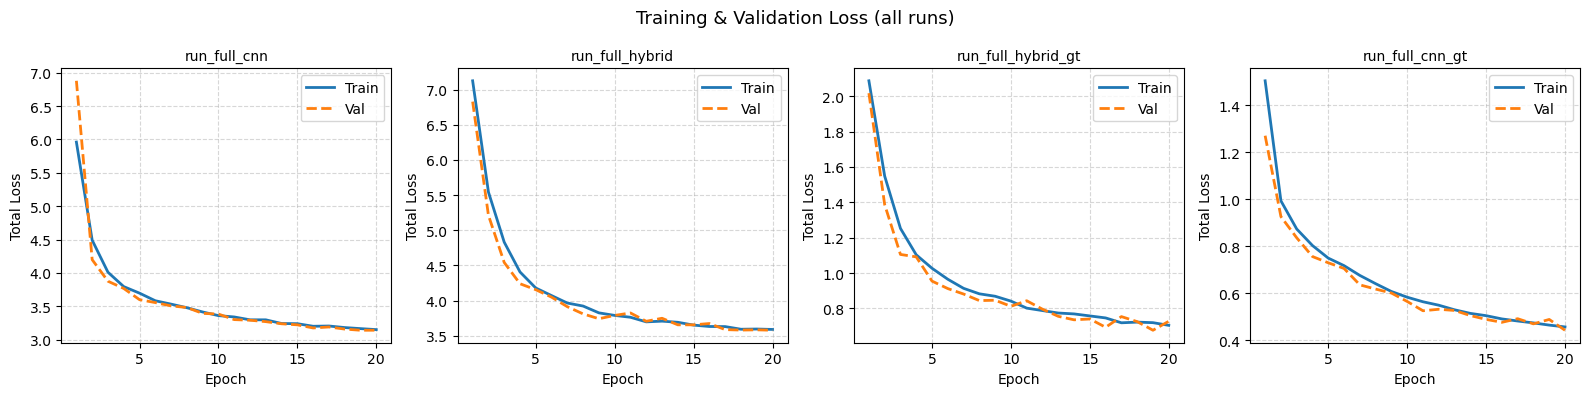
\includegraphics[width=0.8\textwidth, height=0.3\textheight, keepaspectratio]{loss.PNG}\\
  \vspace{0.1em}
  \scriptsize\textcolor{gray}{Training \& validation loss — KD+GT ($\approx$3.1) vs GT-only ($\approx$0.5)}
\end{center}

\vspace{-0.2em}
\centering
\normalsize\textcolor{uoftblue}{\textbf{Thank you! \quad Questions?}}
\end{frame}

\end{document}